% vim: set spell spelllang=en tw=100 et sw=4 sts=4 foldmethod=marker foldmarker={{{,}}} :

\documentclass{beamer}

\usepackage{etex}
\usepackage{tikz}
\usepackage{xcolor}
\usepackage{complexity}
\usepackage{hyperref}
\usepackage{microtype}
\usepackage{amsmath}                   % \operatorname
\usepackage{amsfonts}                  % \mathcal
\usepackage{amssymb}                   % \nexists
\usepackage{gnuplot-lua-tikz}          % graphs
\usepackage[vlined]{algorithm2e} % algorithms
\usepackage{centernot}
\usepackage{mathtools}
\usepackage{listings}
\usepackage{chemfig}

\usetikzlibrary{shapes, arrows, shadows, calc, positioning, fit}
\usetikzlibrary{decorations.pathreplacing, decorations.pathmorphing, shapes.misc}
\usetikzlibrary{tikzmark}

\definecolor{uofguniversityblue}{rgb}{0, 0.219608, 0.396078}

\definecolor{uofgheather}{rgb}{0.356863, 0.32549, 0.490196}
\definecolor{uofgaquamarine}{rgb}{0.603922, 0.72549, 0.678431}
\definecolor{uofgslate}{rgb}{0.309804, 0.34902, 0.380392}
\definecolor{uofgrose}{rgb}{0.823529, 0.470588, 0.709804}
\definecolor{uofgmocha}{rgb}{0.709804, 0.564706, 0.47451}
\definecolor{uofgsandstone}{rgb}{0.321569, 0.278431, 0.231373}
\definecolor{uofgforest}{rgb}{0, 0.2, 0.129412}
\definecolor{uofglawn}{rgb}{0.517647, 0.741176, 0}
\definecolor{uofgcobalt}{rgb}{0, 0.615686, 0.92549}
\definecolor{uofgturquoise}{rgb}{0, 0.709804, 0.819608}
\definecolor{uofgsunshine}{rgb}{1.0, 0.862745, 0.211765}
\definecolor{uofgpumpkin}{rgb}{1.0, 0.72549, 0.282353}
\definecolor{uofgthistle}{rgb}{0.584314, 0.070588, 0.447059}
\definecolor{uofgrust}{rgb}{0.603922, 0.227451, 0.023529}
\definecolor{uofgburgundy}{rgb}{0.490196, 0.133333, 0.223529}
\definecolor{uofgpillarbox}{rgb}{0.701961, 0.047059, 0}
\definecolor{uofglavendar}{rgb}{0.356863, 0.301961, 0.580392}

\tikzset{vertex/.style={draw, circle, inner sep=0pt, minimum size=0.5cm, font=\small\bfseries}}
\tikzset{notvertex/.style={vertex, color=white, text=black}}
\tikzset{plainvertex/.style={vertex}}
\tikzset{vertexc1/.style={vertex, fill=uofgburgundy, text=white}}
\tikzset{vertexc2/.style={vertex, fill=uofgsandstone, text=white}}
\tikzset{vertexc3/.style={vertex, fill=uofgforest, text=white}}
\tikzset{vertexc4/.style={vertex, fill=uofgheather, text=white}}
\tikzset{edge/.style={color=black!50!white}}
\tikzset{bedge/.style={ultra thick}}
\tikzset{edged/.style={color=screengrey, dashed}}
\tikzset{edgel3/.style={color=uofgrose, ultra thick}}

% {{{ theme things
\useoutertheme[footline=authortitle]{miniframes}
\useinnertheme{rectangles}

\setbeamerfont{block title}{size={}}
\setbeamerfont{title}{size=\large,series=\bfseries}
\setbeamerfont{section title}{size=\large,series=\mdseries}
\setbeamerfont{author}{size=\normalsize,series=\mdseries}
\setbeamercolor*{structure}{fg=uofguniversityblue}
\setbeamercolor*{palette primary}{use=structure,fg=black,bg=white}
\setbeamercolor*{palette secondary}{use=structure,fg=white,bg=uofgcobalt}
\setbeamercolor*{palette tertiary}{use=structure,fg=white,bg=uofguniversityblue}
\setbeamercolor*{palette quaternary}{fg=white,bg=black}

\setbeamercolor*{titlelike}{parent=palette primary}

\beamertemplatenavigationsymbolsempty

\setbeamertemplate{title page}
{
    \begin{tikzpicture}[remember picture, overlay]
        \node at (current page.north west) {
            \begin{tikzpicture}[remember picture, overlay]
                \fill [fill=uofguniversityblue, anchor=north west] (0, 0) rectangle (\paperwidth, -2.6cm);
            \end{tikzpicture}
        };

        \node (logo) [anchor=north east, shift={(-0.6cm,-0.6cm)}] at (current page.north east) {
            \includegraphics*[keepaspectratio=true,scale=0.7]{UoG_keyline.pdf}
        };

        \node [anchor=west, xshift=0.2cm] at (current page.west |- logo.west) {
            \begin{minipage}{0.65\paperwidth}\raggedright
                {\usebeamerfont{title}\usebeamercolor[white]{}\inserttitle}\\[0.1cm]
                {\usebeamerfont{author}\usebeamercolor[white]{}\insertauthor}
            \end{minipage}
        };
    \end{tikzpicture}
}

\setbeamertemplate{section page}
{
    \begin{centering}
        \begin{beamercolorbox}[sep=12pt,center]{part title}
            \usebeamerfont{section title}\insertsection\par
        \end{beamercolorbox}
    \end{centering}
}

\newcommand{\frameofframes}{/}
\newcommand{\setframeofframes}[1]{\renewcommand{\frameofframes}{#1}}

\makeatletter
\setbeamertemplate{footline}
{%
    \begin{beamercolorbox}[colsep=1.5pt]{upper separation line foot}
    \end{beamercolorbox}
    \begin{beamercolorbox}[ht=2.5ex,dp=1.125ex,%
        leftskip=.3cm,rightskip=.3cm plus1fil]{author in head/foot}%
        \leavevmode{\usebeamerfont{author in head/foot}\insertshortauthor}%
        \hfill%
        {\usebeamerfont{institute in head/foot}\usebeamercolor[fg]{institute in head/foot}\insertshortinstitute}%
    \end{beamercolorbox}%
    \begin{beamercolorbox}[ht=2.5ex,dp=1.125ex,%
        leftskip=.3cm,rightskip=.3cm plus1fil]{title in head/foot}%
        {\usebeamerfont{title in head/foot}\insertshorttitle}%
        \hfill%
        {\usebeamerfont{frame number}\usebeamercolor[fg]{frame number}\insertframenumber~\frameofframes~\inserttotalframenumber}
    \end{beamercolorbox}%
    \begin{beamercolorbox}[colsep=1.5pt]{lower separation line foot}
    \end{beamercolorbox}
}

% }}}

\title[Solving Hard Graph Problems in Parallel]{Solving Hard Graph Problems \\ in Parallel}
\author[Ciaran McCreesh and Patrick Prosser]{\textbf{Ciaran McCreesh} and Patrick Prosser}

\begin{document}

{
    \usebackgroundtemplate{
        \tikz[overlay, remember picture]
        \node[at=(current page.south), anchor=south, inner sep=0pt]{\includegraphics*[keepaspectratio=true, width=\paperwidth]{background.jpg}};
    }
    \begin{frame}[plain,noframenumbering]
        \titlepage
    \end{frame}
}

\section{\ldots{}Hard Graph Problems\ldots}

\begin{frame}{The Maximum Clique Problem}
    \begin{center}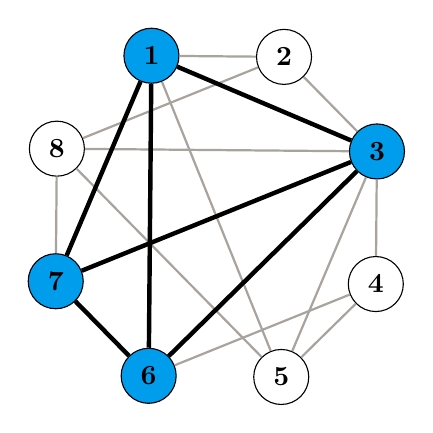
\begin{tikzpicture}
        \newcount \c
        \foreach \n in {1, ..., 8}{
            \c=\n \advance\c by -1 \multiply\c by -360 \divide\c by 8 \advance\c by 112.5
            \ifthenelse{\n = 1 \OR \n = 3 \OR \n = 6 \OR \n = 7}{
                \node[draw, circle, fill=uofgcobalt, inner sep=4pt, font=\bfseries] (N\n) at (\the\c:2.2) {\n};
            }{
                \node[draw, circle, fill=white, inner sep=4pt, font=\bfseries] (N\n) at (\the\c:2.2) {\n};
            }
        }

        \draw [thick, color=uofgsandstone!50] (N1) -- (N2);
        \draw [thick, color=uofgsandstone!50] (N1) -- (N5);
        \draw [thick, color=uofgsandstone!50] (N2) -- (N3);
        \draw [thick, color=uofgsandstone!50] (N2) -- (N8);
        \draw [thick, color=uofgsandstone!50] (N3) -- (N4);
        \draw [thick, color=uofgsandstone!50] (N3) -- (N5);
        \draw [thick, color=uofgsandstone!50] (N3) -- (N8);
        \draw [thick, color=uofgsandstone!50] (N4) -- (N5);
        \draw [thick, color=uofgsandstone!50] (N4) -- (N6);
        \draw [thick, color=uofgsandstone!50] (N5) -- (N8);
        \draw [thick, color=uofgsandstone!50] (N7) -- (N8);

        \draw [ultra thick] (N1) -- (N3);
        \draw [ultra thick] (N1) -- (N6);
        \draw [ultra thick] (N1) -- (N7);
        \draw [ultra thick] (N3) -- (N6);
        \draw [ultra thick] (N3) -- (N7);
        \draw [ultra thick] (N6) -- (N7);
    \end{tikzpicture}\end{center}

\end{frame}

\begin{frame}{Subgraph Isomorphism}
    \begin{center}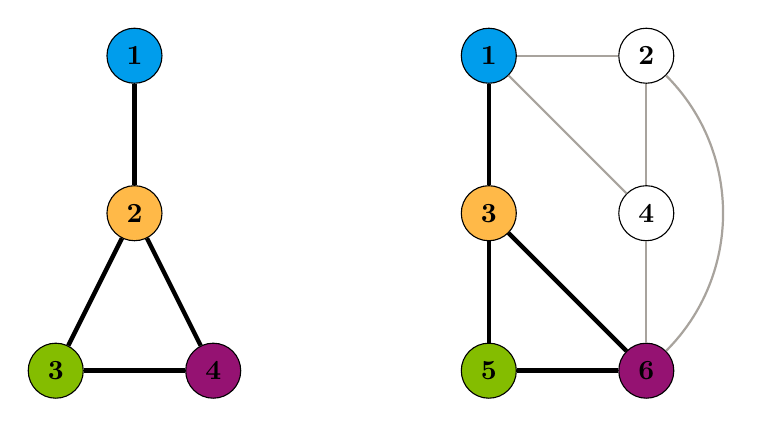
\begin{tikzpicture}
        \node[draw, circle, fill=uofgcobalt, inner sep=4pt, font=\bfseries] (Na) at (1,  0) {1};
        \node[draw, circle, fill=uofgpumpkin, inner sep=4pt, font=\bfseries] (Nb) at (1, -2) {2};
        \node[draw, circle, fill=uofglawn, inner sep=4pt, font=\bfseries] (Nc) at (0, -4) {3};
        \node[draw, circle, fill=uofgthistle, inner sep=4pt, font=\bfseries] (Nd) at (2, -4) {4};

        \draw [ultra thick] (Na) -- (Nb);
        \draw [ultra thick] (Nb) -- (Nc);
        \draw [ultra thick] (Nc) -- (Nd);
        \draw [ultra thick] (Nb) -- (Nd);

        \node[draw, circle, fill=uofgcobalt, inner sep=4pt, font=\bfseries] (N1) at (5.5,  0) {1};
        \node[draw, circle, fill=white, inner sep=4pt, font=\bfseries] (N2) at (7.5,  0) {2};
        \node[draw, circle, fill=uofgpumpkin, inner sep=4pt, font=\bfseries] (N3) at (5.5, -2) {3};
        \node[draw, circle, fill=white, inner sep=4pt, font=\bfseries] (N4) at (7.5, -2) {4};
        \node[draw, circle, fill=uofglawn, inner sep=4pt, font=\bfseries] (N5) at (5.5, -4) {5};
        \node[draw, circle, fill=uofgthistle, inner sep=4pt, font=\bfseries] (N6) at (7.5, -4) {6};

        \draw [thick, color=uofgsandstone!50] (N1) -- (N2);
        \draw [ultra thick] (N1) -- (N3);
        \draw [thick, color=uofgsandstone!50] (N1) -- (N4);
        \draw [thick, color=uofgsandstone!50] (N2) -- (N4);
        \draw [ultra thick] (N3) -- (N5);
        \draw [ultra thick] (N3) -- (N6);
        \draw [thick, color=uofgsandstone!50] (N4) -- (N6);
        \draw [ultra thick] (N5) -- (N6);
        \draw [thick, color=uofgsandstone!50] (N2) to [in=45, out=315] (N6);
    \end{tikzpicture}\end{center}

\end{frame}

\begin{frame}{Maximum Common Subgraph}
    \begin{center}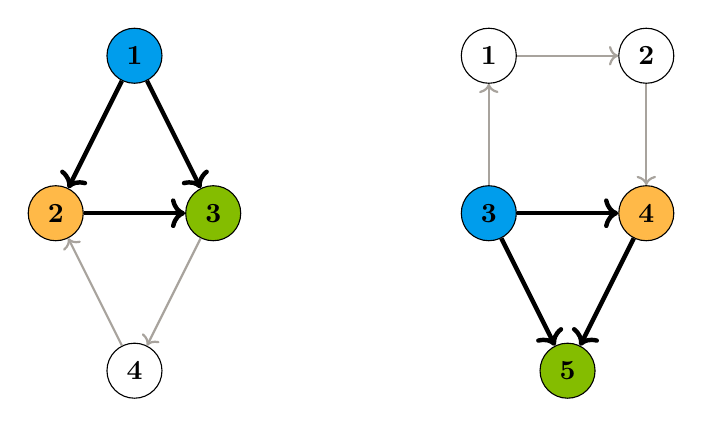
\begin{tikzpicture}%{{{
        \node[draw, circle, fill=uofgcobalt, inner sep=4pt, font=\bfseries] (Ma) at (1, -7.5) {1};
        \node[draw, circle, fill=uofgpumpkin, inner sep=4pt, font=\bfseries] (Mb) at (0, -9.5) {2};
        \node[draw, circle, fill=uofglawn, inner sep=4pt, font=\bfseries] (Mc) at (2, -9.5) {3};
        \node[draw, circle, fill=white, inner sep=4pt, font=\bfseries] (Md) at (1, -11.5) {4};

        \node[draw, circle, fill=white, inner sep=4pt, font=\bfseries] (M1) at (5.5, -7.5) {1};
        \node[draw, circle, fill=white, inner sep=4pt, font=\bfseries] (M2) at (7.5, -7.5) {2};
        \node[draw, circle, fill=uofgcobalt, inner sep=4pt, font=\bfseries] (M3) at (5.5, -9.5) {3};
        \node[draw, circle, fill=uofgpumpkin, inner sep=4pt, font=\bfseries] (M4) at (7.5, -9.5) {4};
        \node[draw, circle, fill=uofglawn, inner sep=4pt, font=\bfseries] (M5) at (6.5, -11.5) {5};

        \draw [->, thick, color=uofgsandstone!50] (Mc) -> (Md);
        \draw [->, thick, color=uofgsandstone!50] (Md) -- (Mb);
        \draw [->, ultra thick] (Ma) -> (Mb);
        \draw [->, ultra thick] (Mb) -> (Mc);
        \draw [->, ultra thick] (Ma) -> (Mc);

        \draw [->, thick, color=uofgsandstone!50] (M1) -> (M2);
        \draw [->, thick, color=uofgsandstone!50] (M2) -> (M4);
        \draw [->, thick, color=uofgsandstone!50] (M3) -> (M1);
        \draw [->, ultra thick] (M3) -> (M4);
        \draw [->, ultra thick] (M3) -> (M5);
        \draw [->, ultra thick] (M4) -> (M5);
    \end{tikzpicture}\end{center}
\end{frame}

\begin{frame}{Maximum Common Connected Subgraph}

    \begin{columns}
        \begin{column}{0.45\textwidth}
            \centering
            \chemfig{*6(-=(-[7]N(-[5]H)(-[7]H))-=-=)}
        \end{column}
        \begin{column}{0.45\textwidth}
            \centering
            \chemfig{*6(-=(-[7]O-[7]N(-[5]H)(-[7]H))-=-=)}
        \end{column}
    \end{columns}

\end{frame}

\section{Solving\ldots}

\begin{frame}{Who Cares?}
    \begin{columns}
        \begin{column}{0.45\textwidth}
            \begin{itemize}
                \item Bioinformatics
                \item Chemistry
                \item Drug design
                \item Computer vision
                \item Pattern recognition
                \item Financial fraud detection
                \item Model checking
                \item Fault detection
            \end{itemize}
        \end{column}
        \begin{column}{0.45\textwidth}
            \begin{itemize}
                \item Law enforcement
                \item Kidney exchange
                \item Social network analysis
                \item Compilers
                \item Diseased cows
                \item Computer algebra
                \item Circuit design
                \item Network design
            \end{itemize}
        \end{column}
    \end{columns}
\end{frame}

\begin{frame}{Practical Algorithms}
    \begin{itemize}
        \item Real-world inputs rarely have nice properties (low treewidth, particular degree
            spreads that are polynomial, etc).

        \item Worst-case performance analysis tells us nothing.

        \item Constant factors matter.
    \end{itemize}
\end{frame}

\begin{frame}{Constraint Models}
    \begin{itemize}
        \item We have some \textbf{variables}, each with a \textbf{domain}, and we want to give each
            variable a value from its domain.
            \begin{itemize}
                \item Clique: a boolean variable for each vertex.
                \item Subgraph isomorphism: a variable for each pattern vertex, with domains being
                    target vertices.
            \end{itemize}
        \item There are \textbf{constraints} between variables.
            \begin{itemize}
                \item Clique: for each pair of non-adjacent vertices, at least one of the two
                    variables must be false.
                \item Subgraph isomorphism: all-different (injectivity), and adjacent pairs of
                    vertices must be mapped to adjacent pairs of vertices.
            \end{itemize}
        \item There is an \textbf{objective}.
            \begin{itemize}
                \item Clique: set as many variables to true as possible.
                \item Subgraph isomorphism: give each variable a value.
            \end{itemize}
    \end{itemize}
\end{frame}

\begin{frame}{Preprocessing}
    \begin{itemize}
        \item We want to ``cross out'' values from domains, until only one value is left in each.
        \item Subgraph isomorphism: high degree vertices cannot be mapped to low degree vertices.
    \end{itemize}
\end{frame}

\begin{frame}{Search}
    \begin{itemize}
        \item Sometimes we have to guess: pick a variable $x$. Then for each value $v_i$ in its
            domain in turn, see what happens if we force $x = v_i$.
        \item There are good heuristics telling us which variable to pick first.
        \item There are heuristics telling us which value to pick first, but this seems to be
            less reliable in general.
    \end{itemize}
\end{frame}

\begin{frame}{Inference}
    \begin{itemize}
        \item After we guess an assignment, we can infer additional deletions. This can have a
            cascade effect.
        \item Sometimes a variable's domain will become empty. Then we fail, and backtrack one level
            and try something else.
    \end{itemize}
\end{frame}

\begin{frame}{Search as a Tree}
    \begin{center}
    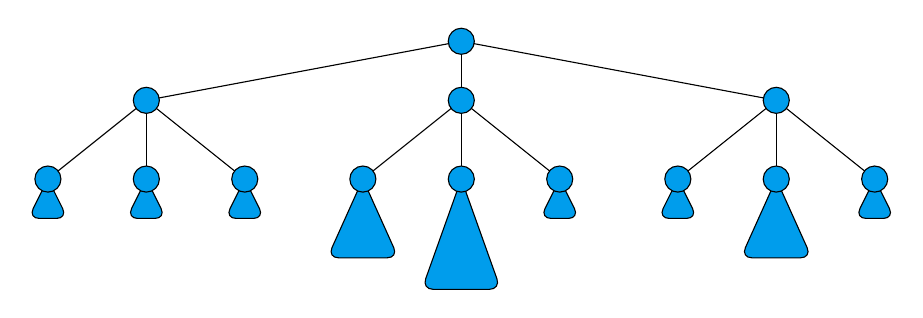
\begin{tikzpicture}%{{{
        \coordinate (R);

        \coordinate (N) at (R);

        \coordinate (N1) at ($(N) + (-4, -0.75)$);
        \coordinate (N2) at ($(N) + ( 0, -0.75)$);
        \coordinate (N3) at ($(N) + ( 4, -0.75)$);

        \foreach \na in {1, ..., 3}{
            \coordinate (N\na 1) at ($(N\na) + (-1.25, -1)$);
            \coordinate (N\na 2) at ($(N\na) + ( 0,    -1)$);
            \coordinate (N\na 3) at ($(N\na) + ( 1.25, -1)$);

            \foreach \nb in {1, ..., 3}{
                \coordinate (N\na\nb t1) at ($(N\na\nb) + (-0.45, -1)$);
                \coordinate (N\na\nb t2) at ($(N\na\nb) + ( 0.45, -1)$);

                \coordinate (N\na\nb s1) at ($(N\na\nb) + (-0.25, -0.5)$);
                \coordinate (N\na\nb s2) at ($(N\na\nb) + ( 0.25, -0.5)$);

                \coordinate (N\na\nb h1) at ($(N\na\nb) + (-0.5, -1.4)$);
                \coordinate (N\na\nb h2) at ($(N\na\nb) + ( 0.5, -1.4)$);
            }
        }

        \foreach \na in {1, ..., 3}{
            \draw (N) -- (N\na);
            \foreach \nb in {1, ..., 3}{
                \draw (N\na) -- (N\na\nb);
            }
        }

        \tikzstyle{t} = [draw, fill, fill=uofgcobalt, rounded corners];

        \draw [t] (N11) -- (N11s1) -- (N11s2) -- cycle;
        \draw [t] (N12) -- (N12s1) -- (N12s2) -- cycle;
        \draw [t] (N13) -- (N13s1) -- (N13s2) -- cycle;

        \draw [t] (N21) -- (N21t1) -- (N21t2) -- cycle;
        \draw [t] (N22) -- (N22h1) -- (N22h2) -- cycle;
        \draw [t] (N23) -- (N23s1) -- (N23s2) -- cycle;

        \draw [t] (N31) -- (N31s1) -- (N31s2) -- cycle;
        \draw [t] (N32) -- (N32t1) -- (N32t2) -- cycle;
        \draw [t] (N33) -- (N33s1) -- (N33s2) -- cycle;

        \tikzstyle{c} = [draw, circle, fill, fill=uofgcobalt];
        \node [c] at (N) { };

        \foreach \na in {1, ..., 3}{
            \node [c] at (N\na) { };

            \foreach \nb in {1, ..., 3}{
                \node [c] at (N\na\nb) { };
            }
        }
    \end{tikzpicture}%}}}
    \end{center}

\end{frame}

\begin{frame}{Branch and Bound}

    \begin{center}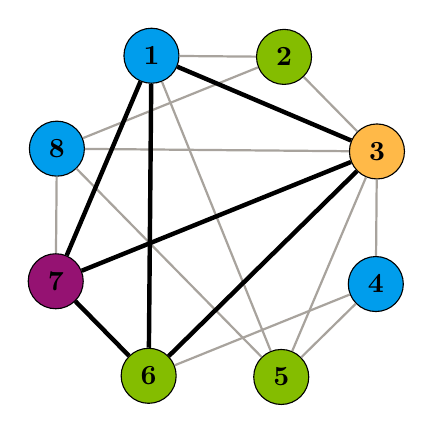
\begin{tikzpicture}
        \newcount \c
        \foreach \n in {1, ..., 8}{
            \c=\n \advance\c by -1 \multiply\c by -360 \divide\c by 8 \advance\c by 112.5
            \ifthenelse{\n = 1 \OR \n = 4 \OR \n = 8}{
                \node[draw, circle, fill=uofgcobalt, inner sep=4pt, font=\bfseries] (N\n) at (\the\c:2.2) {\n};
            }{}
            \ifthenelse{\n = 2 \OR \n = 5 \OR \n = 6}{
                \node[draw, circle, fill=uofglawn, inner sep=4pt, font=\bfseries] (N\n) at (\the\c:2.2) {\n};
            }{}
            \ifthenelse{\n = 3}{
                \node[draw, circle, fill=uofgpumpkin, inner sep=4pt, font=\bfseries] (N\n) at (\the\c:2.2) {\n};
            }{}
            \ifthenelse{\n = 7}{
                \node[draw, circle, fill=uofgthistle, inner sep=4pt, font=\bfseries] (N\n) at (\the\c:2.2) {\n};
            }{}
        }

        \draw [thick, color=uofgsandstone!50] (N1) -- (N2);
        \draw [thick, color=uofgsandstone!50] (N1) -- (N5);
        \draw [thick, color=uofgsandstone!50] (N2) -- (N3);
        \draw [thick, color=uofgsandstone!50] (N2) -- (N8);
        \draw [thick, color=uofgsandstone!50] (N3) -- (N4);
        \draw [thick, color=uofgsandstone!50] (N3) -- (N5);
        \draw [thick, color=uofgsandstone!50] (N3) -- (N8);
        \draw [thick, color=uofgsandstone!50] (N4) -- (N5);
        \draw [thick, color=uofgsandstone!50] (N4) -- (N6);
        \draw [thick, color=uofgsandstone!50] (N5) -- (N8);
        \draw [thick, color=uofgsandstone!50] (N7) -- (N8);

        \draw [ultra thick] (N1) -- (N3);
        \draw [ultra thick] (N1) -- (N6);
        \draw [ultra thick] (N1) -- (N7);
        \draw [ultra thick] (N3) -- (N6);
        \draw [ultra thick] (N3) -- (N7);
        \draw [ultra thick] (N6) -- (N7);
    \end{tikzpicture}\end{center}

    \begin{itemize}
        \item For optimisation: keep track of the best solution we've found so far. If we can show
            we can't beat it, backtrack immediately.
    \end{itemize}

\end{frame}

\begin{frame}{Backjumping}

\end{frame}

\begin{frame}{Implied Constraints for Subgraph Isomorphism}

\end{frame}

\section{\ldots{}In Parallel}

\begin{frame}{Bit-Parallel Inference}

\end{frame}

\begin{frame}{Thread-Parallel Tree Search}

\end{frame}

\begin{frame}{Parallel Search Order Matters}

\end{frame}

\begin{frame}{Parallel Backjumping}

\end{frame}

\begin{frame}{Safety and Reproducibility}

    \begin{itemize}
        \item My ``wish list'':
            \begin{enumerate}
                \item Parallel search should not be substantially slower than sequential search.
                \item Adding more processors should not make things substantially worse.
                \item Running the same program twice on the same hardware should give similar
                    runtimes.
            \end{enumerate}
        \item This is surprisingly tricky and controversial.
    \end{itemize}

\end{frame}

\section{Works in Progress}

\begin{frame}{Describing and Implementing Parallel Search}

    \begin{itemize}
        \item Implementing safe and reproducible parallel search by hand, even just for multi-core,
            is painful.
        \item Current high level approaches don't offer the properties we need.
        \item Is there a better way?
    \end{itemize}

\end{frame}

\begin{frame}{Symmetries}

    \begin{itemize}
        \item Some graphs have known symmetries. Can we exploit this?

            \begin{itemize}
                \item In some ways, maximum clique is just a completely symmetric version of maximum
                    common subgraph.
            \end{itemize}

        \item What about if we have to detect the symmetries ourselves dynamically?
    \end{itemize}

\end{frame}

\begin{frame}{Explaining Failures}

    \begin{itemize}
        \item Backjumping works because when we fail, we work out why, and use that to backtrack
            further.

        \item But then we throw that information away\ldots
    \end{itemize}

\end{frame}

\begin{frame}{Hard Subgraph Isomorphism Instances}

    \only<1> {
        \begin{itemize}
            \item We like having lots of instances, to make sure we don't overfit algorithm parameters.

            \item How do we randomly create subgraph isomorphism instances?
        \end{itemize}
    }

    \only<2> {

    }

\end{frame}

\begin{frame}{Hybrid Graph Modelling and Optimisation}

\end{frame}

\begin{frame}[plain,noframenumbering,b]
    \begin{tikzpicture}[remember picture, overlay]
        \node at (current page.north west) {
            \begin{tikzpicture}[remember picture, overlay]
                \fill [fill=uofguniversityblue, anchor=north west] (0, 0) rectangle (\paperwidth, -1.7cm);
            \end{tikzpicture}
        };

        \node (logo) [anchor=north east, shift={(-0.3cm,-0.2cm)}] at (current page.north east) {
            \includegraphics*[keepaspectratio=true,scale=0.55]{UoG_keyline.pdf}
        };
    \end{tikzpicture}

    \begin{center}
        \url{http://dcs.gla.ac.uk/~ciaran} \\
        \href{mailto:c.mccreesh.1@research.gla.ac.uk}{\nolinkurl{c.mccreesh.1@research.gla.ac.uk}}
        \\ [1cm]
    \end{center}
\end{frame}

\end{document}

